	\chapter{Planificación y Gestión del Proyecto}
	\section{Cronograma}
	\begin{figure}[h]
		\centering
		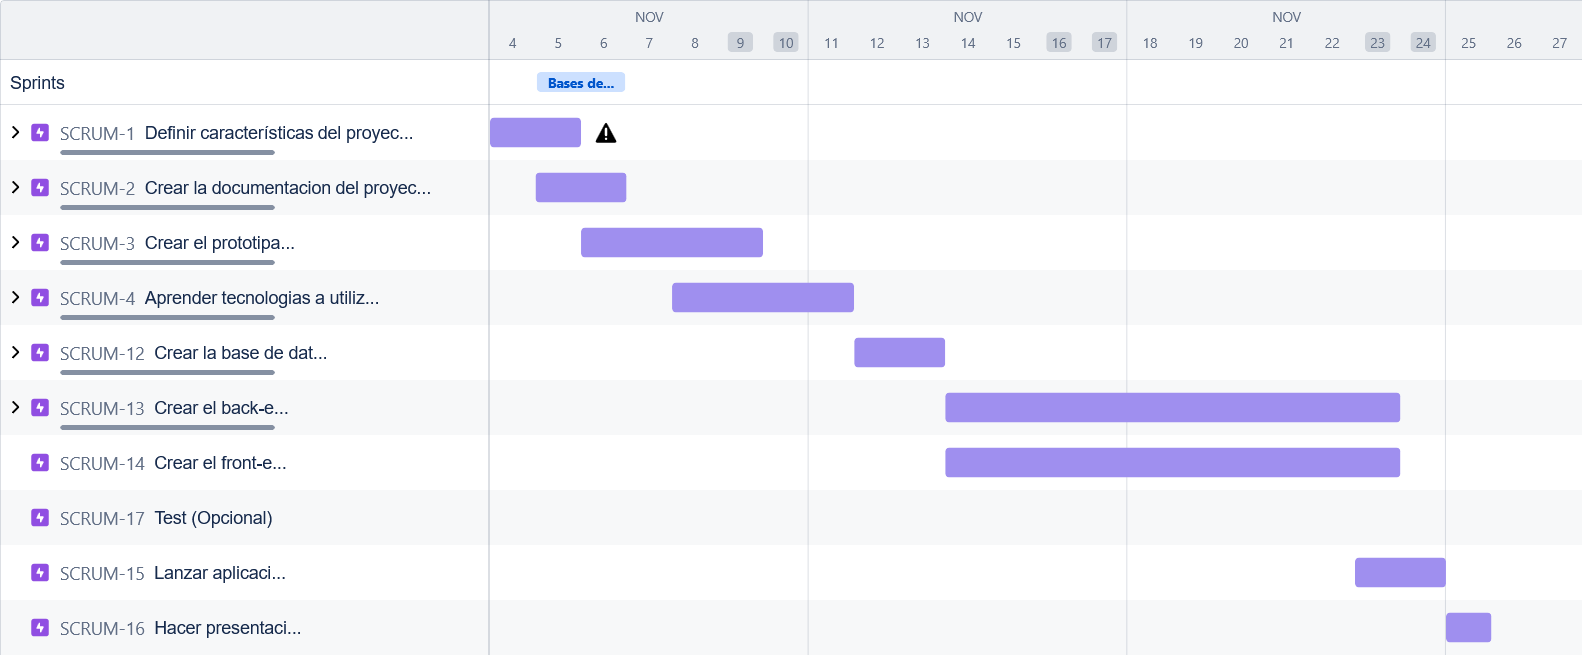
\includegraphics[width=1\linewidth]{./images/proyecto_final_ingr_2024-11-05_11.32am}
		\caption{Cronograma del Proyecto obtenido de JIRA}
	\end{figure}
	
	\section{Recursos y Roles}
	Recursos:
	\begin{itemize}
		\item 1 Líder de Proyecto
		\item 2 Desarrolladores
	\end{itemize}

	Roles: 
	\begin{itemize}
		\item Líder de Proyecto: Alejandro Macías Fonseca
		\item Desarrollador Backend: Alejandro Macías Fonseca
		\item Desarrollador Backend: David Mata Guerra
		\item Desarrollador Frontend: Alexis Emilio Cárdenas Camacho
		\item Desarrollador Frontend: Gabriel Juárez Ramírez
	\end{itemize}
	
	\section{Control de Versiones}
	El control de versiones se llevó a cabo utilizando Git y GitHub. 
		\begin{center}
		
\includegraphics[width=0.3\linewidth]{./images/gitlogo.png}
		
\includegraphics[width=0.3\linewidth]{./images/github_logo.png}
	\end{center}
	Se crearon dos repositorios :
	\begin{itemize}
		\item 	Backend: \url{https://github.com/dmataguerra/proyecto_final_ing_requerimientos_back}
		\item   Frontend: \url{POR DEFINIR}	
	\end{itemize}
